% Typeset with LaTeX format
% Using AMS extensions for mathematical formatting

%	The 'myarticle' class gives me a smaller title size
%	This class should appear as 'article'
%	in any submitted source file, so that others can
%	properly format it.  Please change if it is not correct.
%  	I use the 'leqno' option, for left-handed equation numbers.
\documentclass[leqno,11pt]{article}
%	To get all the formal devices, I usually use
%	all of 'amsmath', 'amssymb', and 'amsthm'.
%	There may also appear the packages
%	'setspace' (for double-spacing)
%	and 'mylogic' (for personal margins, headers, commands, etc.)
%	These should NOT appear in any submitted source file.
%	Please remove them if still here upon submission.
\usepackage{amsmath,amssymb,amsthm,amscd,amsxtra,latexsym}
\usepackage{enumerate}
\usepackage{graphicx}
\usepackage{hanging}
\usepackage[colorlinks=true,urlcolor=blue,linkcolor=black]{hyperref}
\usepackage{color}
\usepackage{tikz}

%---------------------------------------------
%       OPTIONAL:  PAGE SPACING HERE
%---------------------------------------------

%\usepackage{setspace}
%	The following line may be commented out
% 	If so, it can be deleted without affecting anything.
%	I use the command (with the 'setspace.sty' package)
%	for alternative formatting (also \doublespacing).
%	If this line is commented out, and 'setspace' is not in use,
%	the document formats as usual for its class.
%%\onehalfspacing

%---------------------------------------------
%       PAGE FORMAT (BORDERS/HEADERS)
%---------------------------------------------

%	Page format commands:
%	Override normal article margins,
%	making the margins smaller
\setlength{\textwidth}{6.5in}
\setlength{\textheight}{8.75in}
\setlength{\oddsidemargin}{0in}
\setlength{\evensidemargin}{0in}
\setlength{\topmargin}{-0.25in}

%---------------------------------------------
%       DEFINED COMMANDS
%---------------------------------------------

% A command for   'cardinality-of-XX' := |XX|
\newcommand{\card}[1]%
	{\ensuremath{\left| #1 \right|}}

% A command for 'set containing XX' := {XX}
\newcommand{\set}[1]%
	{\ensuremath{ \{ #1 \} }}

%	The 'such that' bar for set notation
\newcommand{\suth}{\ensuremath{ \,|\, }}

% A command for primes (')
\newcommand{\prm}%
	{\ensuremath{^{\prime}}}
		
% a command for double primes ('')
\newcommand{\pprm}%
	{\ensuremath{^{\prime \prime}}}

% A command for the Kleene star
\newcommand{\str}%
	{\ensuremath{^{\star}}}

% a command for the double star
\newcommand{\sstr}%
	{\ensuremath{^{\star\star}}}

% a command for question-numbers
\newcommand{\qn}[1]%
	{\noindent \textbf{[ #1 ]}\quad}
	
%---------------------------------------------
%       DOC STARTS HERE
%---------------------------------------------

\begin{document}

\begin{center}
{\large
\textbf{Computation Theory (CS 170), Summer 2023} \\
\rule{0pt}{1em} \textbf{Assignment 02; due 11:59 PM Eastern, Wednesday 14th June 2023}
}
\\
\hrulefill
\end{center}

\noindent 
Answer each of the following three questions to the best of your ability.  \textbf{Make sure that your
submission follows the formatting guidelines given at the end of this document.}

\vspace{4pt}\noindent 
You can find instructions for how to submit your work to Gradescope on the class website:
\begin{center}
	\href{https://canvas.tufts.edu/courses/44798/pages/how-to-submit-homework}
	{https://canvas.tufts.edu/courses/44798/pages/how-to-submit-homework}
\end{center}
 
\hrulefill 

\vspace{10pt}

\qn{1} (\emph{5 pts.}) Consider the following language on binary alphabet $\Sigma =
\set{\texttt{0},\, \texttt{1}}$:
\[
	L = \set{w = \texttt{0}^i \texttt{1}^j \suth (j - i) \text{ is a non-negative even number}} 
\]
Examples of strings in $L$ are $\varepsilon$, \texttt{0111}, \texttt{00011111}, etc. Note that $\varepsilon \in
L$ since $\varepsilon = \texttt{0}^0 \texttt{1}^0$, and $(0 - 0) = 0$, a non-negative even number.  Also note
that any string consisting only of an even number of \texttt{1}'s is also a member of $L$, since if 
$w = \texttt{1}^j$ and $j$ is even, so is $(j - 0)$.

\vspace{6pt} \noindent  
Prove that this language is non-regular, using the Pumping Lemma.



Proof:

For the sake of contradiction assume L is regular so by the Pumping Lemma some pumping length p exists.

Consider s = ${\texttt{0}^p{1}^p}\varepsilon$ L so ${|s| = 2p \geq p}$


So by the Pumping Lemma we can divide s = xyz such that ${|y| \geq 0}$ and ${|xy| \leq p}$

So ${y = 0^k}$ for some ${k > 0}$

But ${xy^2z = 0^{p+k}1^p = 0^{i+k}1^j}$ which would produce a negative number since ${(i+k) > j}$ so ${xy^2z \not\mathrel{\varepsilon} L}$

So by this contradiction we can conclude L is non-regular 

\vspace{16pt}

\qn{2} (\emph{5 pts.}) Let the alphabet $\Sigma = \set{\texttt{a},\, \texttt{b}}$.  Define the two
following languages:
\begin{align*}
	L_1 &= \set{\texttt{a}^n \texttt{ba}^n \suth n \geq 1} \\
	L_2 &= \set{w_1 \texttt{a}^n \texttt{ba}^n w_2 \suth n \geq 1 \texttt{ and } w_1,\, w_2 \in \Sigma\str}
\end{align*}
Examples of strings in $L_1$ include: \texttt{aba}, \texttt{aabaa}, \texttt{aaabaaa}, \texttt{aaaabaaaa}, etc. 

\vspace{6pt}\noindent 
Examples of strings in $L_2$ include: \texttt{aba}, \texttt{baabaab}, \texttt{bbaaabaaa}, \texttt{abaaaabaaaab}, etc. 
(since the strings $w_1$ and $w_2$ that form the front and back can be any combination of \texttt{a}'s and
\texttt{b}'s).

\begin{enumerate} [\quad a.] 


   \item Show that $L_2$ is regular, by giving a DFA or NFA for it.

   \begin{center}
\begin{tikzpicture}[scale=0.2]
\tikzstyle{every node}+=[inner sep=0pt]
\draw [black] (10.3,-24.3) circle (3);
\draw (10.3,-24.3) node {$q0$};
\draw [black] (34,-24.3) circle (3);
\draw (34,-24.3) node {$q1$};
\draw [black] (34,-39.9) circle (3);
\draw (34,-39.9) node {$q2$};
\draw [black] (10.3,-39.9) circle (3);
\draw (10.3,-39.9) node {$q3$};
\draw [black] (10.3,-39.9) circle (2.4);
\draw [black] (3.1,-24.3) -- (7.3,-24.3);
\fill [black] (7.3,-24.3) -- (6.5,-23.8) -- (6.5,-24.8);
\draw [black] (9.27,-21.495) arc (227.8845:-60.1155:2.25);
\draw (11.23,-17) node [above] {$b$};
\fill [black] (11.9,-21.78) -- (12.81,-21.52) -- (12.07,-20.85);
\draw [black] (34.621,-21.377) arc (195.74698:-92.25302:2.25);
\draw (39.13,-18.5) node [above] {$a$};
\fill [black] (36.7,-23.01) -- (37.6,-23.28) -- (37.33,-22.32);
\draw [black] (13.3,-24.3) -- (31,-24.3);
\fill [black] (31,-24.3) -- (30.2,-23.8) -- (30.2,-24.8);
\draw (22.15,-24.8) node [below] {$a$};
\draw [black] (31.501,-38.269) arc (-133.27052:-226.72948:8.473);
\fill [black] (31.5,-38.27) -- (31.26,-37.36) -- (30.58,-38.08);
\draw (28.34,-32.1) node [left] {$b$};
\draw [black] (31,-39.9) -- (13.3,-39.9);
\fill [black] (13.3,-39.9) -- (14.1,-40.4) -- (14.1,-39.4);
\draw (22.15,-39.4) node [above] {$a$};
\draw [black] (36.673,-25.624) arc (53.04981:-53.04981:8.104);
\fill [black] (36.67,-25.62) -- (37.01,-26.5) -- (37.61,-25.71);
\draw (40.41,-32.1) node [right] {$b$};
\draw [black] (11.23,-42.74) arc (45.8699:-242.1301:2.25);
\draw (8.67,-47.26) node [below] {$a,\mbox{ }b$};
\fill [black] (8.61,-42.37) -- (7.7,-42.59) -- (8.41,-43.29);
\end{tikzpicture}
\end{center}

   \item Show that $L_1$ is not regular, using the Pumping Lemma to prove it.
\end{enumerate} 

Proof:

For the sake of contradiction assume $L_1$ is regular so by the Pumping Lemma some pumping length p exists.

Consider s = ${\texttt{a}^p{b}{a}^p}\varepsilon$ L so ${|s| = 2p + 1 \geq p}$


So by the Pumping Lemma we can divide s = xyz such that ${|y| \geq 0}$ and ${|xy| \leq p}$

So ${y = a^k}$ for some ${k > 0}$

But ${xy^2z = \texttt{a}^{p+k}{b}{a}^p = \texttt{a}^{n+k}{b}{a}^n }$ which would be uneven so ${xy^2z \not\mathrel{\varepsilon} L}$

So by this contradiction we can conclude $L_1$ is non-regular 

\vspace{16pt}

\qn{3} (\emph{5 pts.}) Let our alphabet be $\Sigma = \set{ \texttt{0},\, \texttt{1},\, \texttt{-},\, \texttt{=}}$,
and let our language be the set of strings expressing correct arithmetic differences between binary numbers.
(Here, we will define a binary number as any non-empty binary string; leading zeros are allowed.  Thus, for
example, both \texttt{11101} and \texttt{0011101} are allowed, as each is a binary number, equal to 29.):
\[
	L_{*} = \set{w_1 \texttt{=} w_2 \texttt{-} w_3 \suth \text{$w_1$, $w_2$, and $w_3$ are binary numbers, and
	$w_2$ is the sum of $w_1$ and $w_3$}}
\]
Show that this language is not regular, using the Pumping Lemma to prove it.

Proof:

For the sake of contradiction assume $L_{*}$ is regular so by the Pumping Lemma some pumping length p exists.

Consider s = ${\texttt{(001}^p=010-001)}\varepsilon$ L so ${|s| = p + 8 \geq p}$


So by the Pumping Lemma we can divide s = xyz such that ${|y| \geq 0}$ and ${|xy| \leq p}$

So ${y = 001^k}$ for some ${k > 0}$

But ${xy^2z = \texttt({001}^2=010-001)= \texttt(001001=010-001)}$ which is an incorrect expression so ${xy^2z \not\mathrel{\varepsilon} L_{*}}$

So by this contradiction we can conclude $L_{*}$ is non-regular 


 \pagebreak 

\noindent 
\textbf{Format requirements}: work should correspond to the following guidelines:
\begin{itemize}  

	\item Work must be in type-written format, with any diagrams rendered using software to produce
		professional-looking results.  No hand-written or hand-drawn work will be graded.
		
	\item Work must be submitted in PDF format to Gradescope.

\end{itemize}

\vspace{4pt}\noindent 
You can find links to information about using LaTeX to produce type-written mathematical work,\footnote{LaTeX
was used to produce this document.}  on the class website:
\begin{center}
	\href{https://canvas.tufts.edu/courses/44798/pages/latex-document-preparation}
	{https://canvas.tufts.edu/courses/44798/pages/latex-document-preparation}
\end{center}
While you can use any drawing/layout program to produce images, there is a handy web-based tool for drawing
finite-state diagrams for DFA/NFA that produces nice results (the image in this assignment was generated using
that tool, exporting the code for the image to LaTeX for inclusion):
\begin{center}
	\href{http://madebyevan.com/fsm/}{http://madebyevan.com/fsm/}
\end{center}
 
\end{document}
 
